% Paper #3 FIG-1: Schur-pipeline schematic
% Build standalone:
%   pdflatex paper3_fig1.tex
\documentclass[border=4pt]{standalone}
\usepackage{tikz}
\usetikzlibrary{arrows.meta,positioning,shapes,backgrounds}
\begin{document}
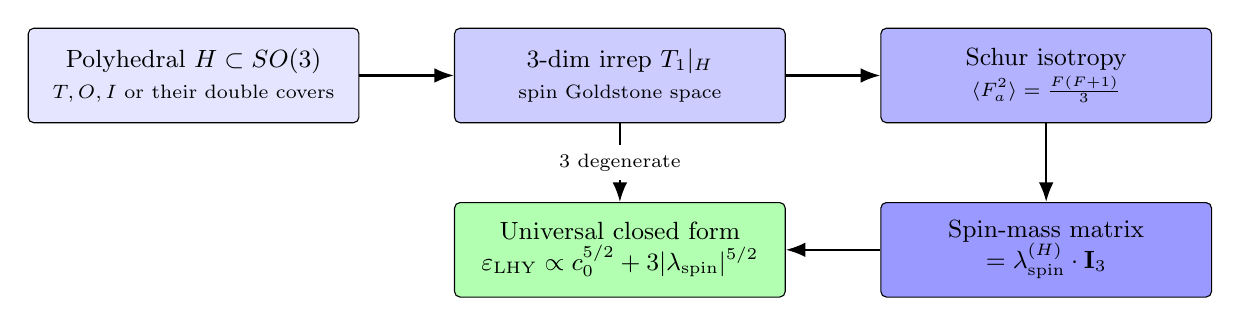
\begin{tikzpicture}[
    node distance=10mm,
    box/.style={draw, rounded corners=2pt, minimum width=42mm,
                minimum height=12mm, align=center, font=\small},
    arrow/.style={-{Latex[length=2.5mm]}, thick},
]
% Step 1
\node[box, fill=blue!10] (group) {Polyhedral $H \subset SO(3)$\\
    \scriptsize $T, O, I$ or their double covers};
% Step 2
\node[box, fill=blue!20, right=12mm of group] (irrep) {3-dim irrep $T_1|_H$\\
    \scriptsize spin Goldstone space};
% Step 3
\node[box, fill=blue!30, right=12mm of irrep] (schur) {Schur isotropy\\
    \scriptsize $\langle F_a^2\rangle = \frac{F(F+1)}{3}$};
% Step 4
\node[box, fill=blue!40, below=10mm of schur] (eom) {Spin-mass matrix\\
    $= \lambda_{\rm spin}^{(H)} \cdot \mathbf{I}_3$};
% Step 5
\node[box, fill=green!30, below=10mm of irrep] (closed) {Universal closed form\\
    $\varepsilon_{\rm LHY} \propto c_0^{5/2} + 3|\lambda_{\rm spin}|^{5/2}$};

% Arrows
\draw[arrow] (group) -- (irrep);
\draw[arrow] (irrep) -- (schur);
\draw[arrow] (schur) -- (eom);
\draw[arrow] (eom) -- (closed);
\draw[arrow] (irrep) -- (closed) node[midway,fill=white,font=\scriptsize]
    {3 degenerate};

\end{tikzpicture}
\end{document}
